\chapter{Технологический раздел}

\section{Язык программирования}
В качестве языка программирований выбран язык высокого уровня JavaScript.

\section{Примеры кода}

\begin{lstlisting}[caption={Программная модель клиента}]
function SourceOfInformation(min, max) {
  let self = this;
  
  self.min = min;
  self.max = max;

  let isRequest = false;

  let timeNewOrder = randFromMinToMax(self.min, self.max);

  self.isRequest = function(nowTime) {
    if (nowTime >= timeNewOrder && !isRequest)  {
      isRequest = true;
      timeNewOrder += randFromMinToMax(self.min, self.max);
    }

    return isRequest;
  }

  self.reset = function() {
    isRequest = false;
  }
}
\end{lstlisting}

\begin{lstlisting}[caption={Программная модель компьютера}]
function Store(time) {
  let self = this;
  
  self.time = time;

  let orders = [];

  self.pushOrder = function(nowTime) {
    orders.push(nowTime);
  }

  self.run = function(nowTime) {
    //orders.sort((a, b) => a - b);

    let i = 0;
    while(orders[i] + self.time < nowTime) {
      orders.shift();
      ++i;
    }

    return i;
  }
}
\end{lstlisting}

\begin{lstlisting}[caption={Программная модель оператора}]
function ServiceUnit(min, max, store) {
  let self = this;
  
  self.min = min;
  self.max = max;
  self.store = store;

  let isFree = false;
  
  let timeNewWork = randFromMinToMax(self.min, self.max);

  self.isFree = function(nowTime) {
    if (nowTime >= timeNewWork && !isFree) {
      isFree = true;
      self.store.pushOrder(nowTime);  
    } 

    return isFree;
  }

  self.pushWork = function(nowTime) {
    isFree = false;
    timeNewWork = nowTime + randFromMinToMax(self.min, self.max);
  }
} 

\end{lstlisting}


\section{Взаимодействие с пользователем}

Взаимодейсвтие с пользователем осуществляется через html страницы, открытые в браузере.

\begin{figure}
  \centering
  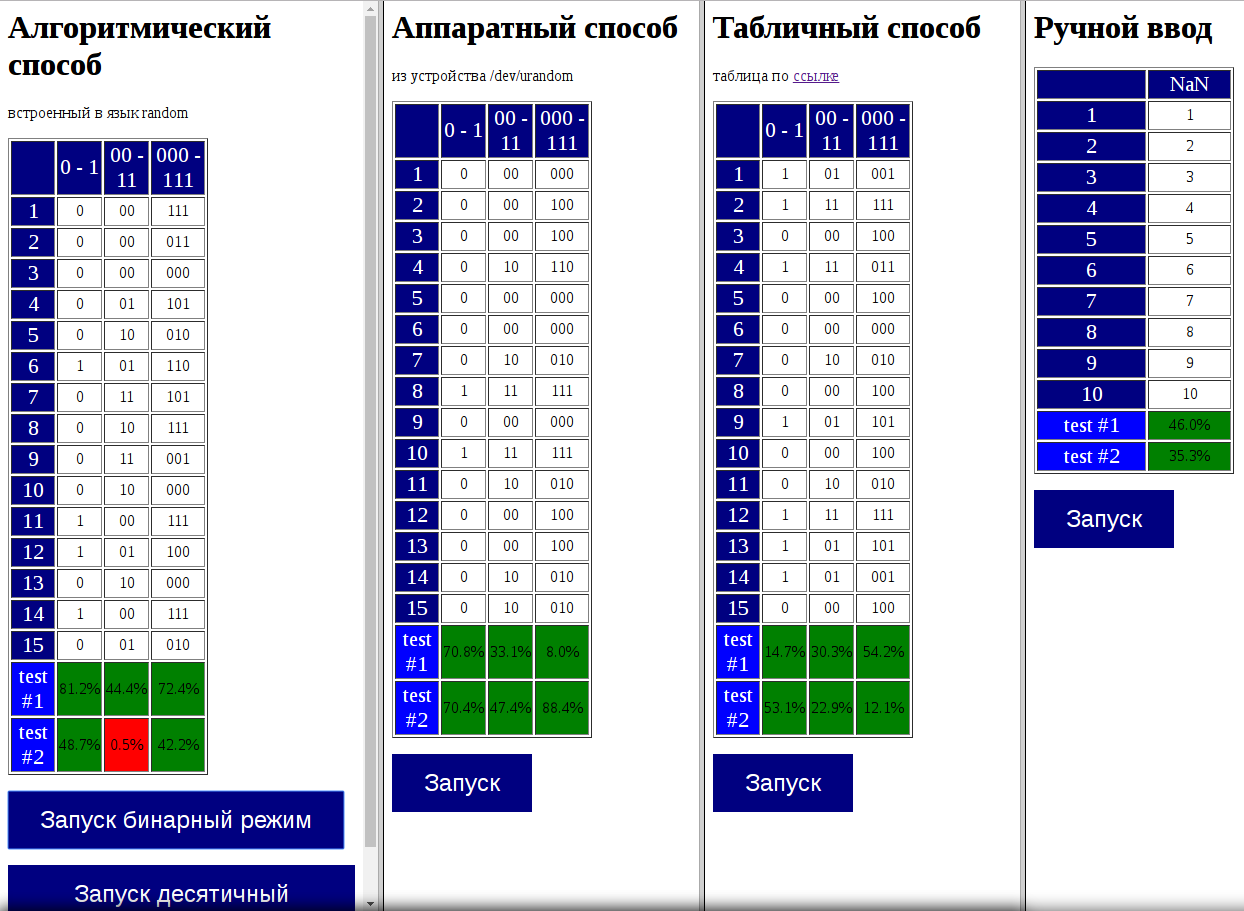
\includegraphics[scale=0.8]{screen1.png}
  \caption{Настройка параметров модели}
\end{figure}

\begin{figure}
  \centering
  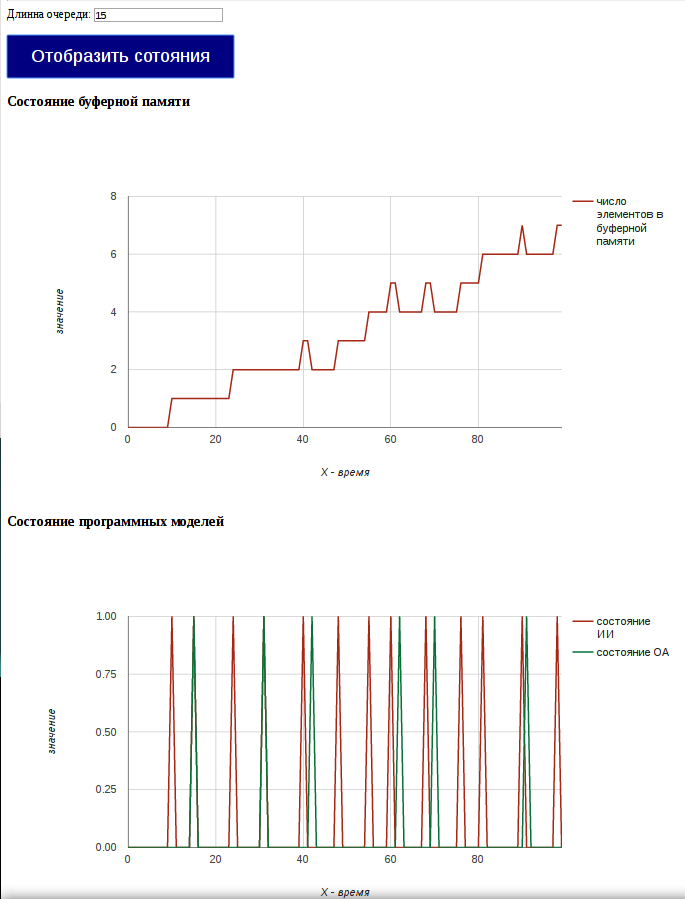
\includegraphics[scale=0.8]{screen2.png}
  \caption{Результаты}
\end{figure}